\section{mr::progressbuffer Struct Reference}
\label{structmr_1_1progressbuffer}\index{mr::progressbuffer@{mr::progressbuffer}}
{\tt \#include $<$mr\-Stream.h$>$}

Inheritance diagram for mr::progressbuffer::\begin{figure}[H]
\begin{center}
\leavevmode
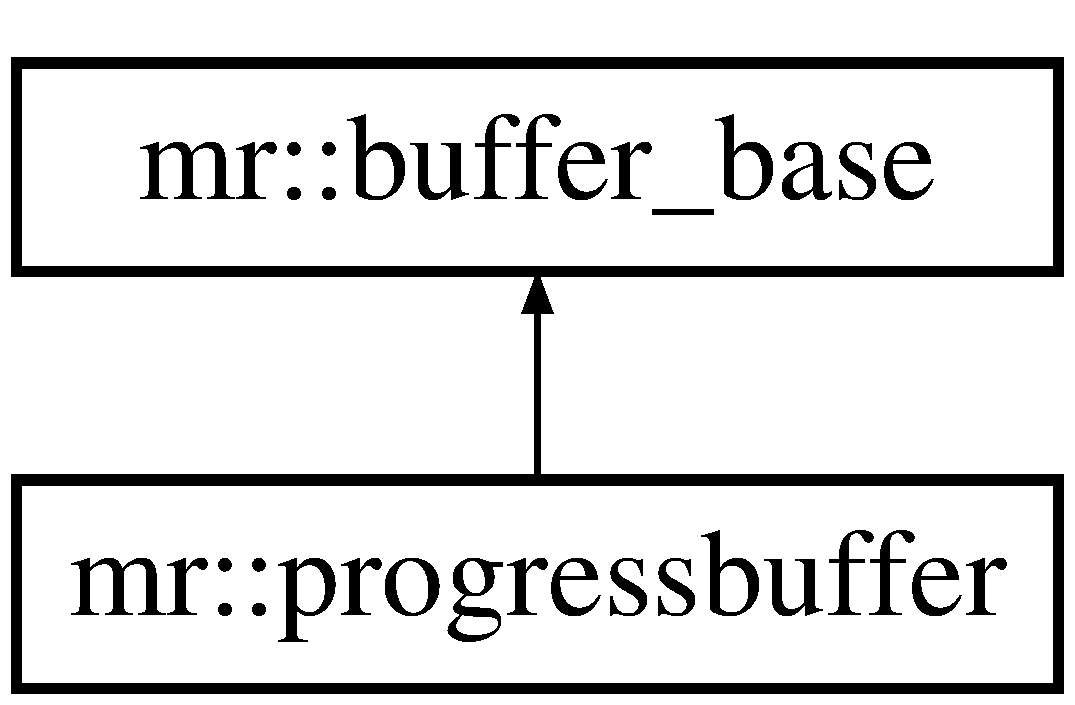
\includegraphics[height=2cm]{structmr_1_1progressbuffer}
\end{center}
\end{figure}
\subsection*{Public Member Functions}
\begin{CompactItemize}
\item 
{\bf progressbuffer} ()
\item 
virtual void {\bf print} (const char $\ast$const s)
\begin{CompactList}\small\item\em virtual function to print string out \item\end{CompactList}\end{CompactItemize}


\subsection{Constructor \& Destructor Documentation}
\index{mr::progressbuffer@{mr::progressbuffer}!progressbuffer@{progressbuffer}}
\index{progressbuffer@{progressbuffer}!mr::progressbuffer@{mr::progressbuffer}}
\subsubsection{\setlength{\rightskip}{0pt plus 5cm}mr::progressbuffer::progressbuffer ()\hspace{0.3cm}{\tt  [inline]}}\label{structmr_1_1progressbuffer_a0}




\subsection{Member Function Documentation}
\index{mr::progressbuffer@{mr::progressbuffer}!print@{print}}
\index{print@{print}!mr::progressbuffer@{mr::progressbuffer}}
\subsubsection{\setlength{\rightskip}{0pt plus 5cm}virtual void mr::progressbuffer::print (const char $\ast$const {\em s})\hspace{0.3cm}{\tt  [inline, virtual]}}\label{structmr_1_1progressbuffer_a1}


virtual function to print string out 



Implements {\bf mr::buffer\_\-base} {\rm (p.\,\pageref{structmr_1_1buffer__base_a3})}.

The documentation for this struct was generated from the following file:\begin{CompactItemize}
\item 
{\bf mr\-Stream.h}\end{CompactItemize}
